\documentclass{article}
\usepackage{graphicx,verbatim}

\title{ResTracker}
\author{Team 16\\Stephanie Fuller (sfuller@wpi.edu)\\Jamie Bliss (jebliss@wpi.edu)\\Sam
LaFleche (shl@wpi.edu)}

\begin{document}

\maketitle

\section{Description}
As it currently stands the WPI administration does not have a good tool for
managing what rooms have been reserved by student organizations. Room
reservations are often lost, forgotten about, or double booked leading to
frustration on the part of organizations and difficulty running events. Having a
single database where room reservations could be tracked, added and deleted
would mitigate this problem.

\section{ER Model}
\scalebox{.42}{\includegraphics[angle=90]{ERmodel.eps}}

\section{Requirements}

\begin{itemize}
\item Users are broken up into Administrators, Super Administrators, Anonymous Users, Students, and Groups
\item All users have names, email addresses, and passwords.
\item Students also have a graduation year and major(s).
\item Administrators have titles and Super Administrator privileges or not. 
\item Groups have descriptions and what class (class 1, class 2, class 3, etc.).
\item Events have a name, description, ID, and expected size.
\item Events have sponsoring groups, name, description, and room reservation(s).
\item There are rooms. Rooms have buildings, room numbers, and occupancy.
\item There is equipment. Equipment is a type of equipment.
\item Equipment can be in rooms and can be used for events.
\item When equipment is in a room there is a quantity.
\item A reservation shall include who booked it, what administrator
approved it (if any), when it was booked, when it is being reserved,
and the event it is for.
\item The system notifies the group and user which created it with any
changes to an event or reservation.
\item All changes (eg additions, deletions, and mutations) shall be
logged, including the user who made the change, the event that was
changed, and the old and new data.
\item The database shall be usable by multiple users at once.
\item The database shall have a UI capable of showing relevant information.
\item For each reservation the student who made the reservation must
be a member of the group the reservation is for.
\item Events can have any number of comments on them, including none.
\item Comments must be on exactly one event.
\item Each comment is made only by one user.
\item Events are run by one or more clubs. There cannot be an event run by no
club, but more than one club can run the event. This is as is currently done for
events at WPI.  
\item Groups can run any number of events including none. New clubs can have not
run any events yet. 
\item Events may or may not use equipment.
\item Equipment may or may not be used.
\item Students can make reservations, but do not have to do so.
\item Rooms may be reserved, but do not have to be.
\item Rooms cannot be booked for more than one event at the same time. 
\item Events can be in public, non-reservable places.
\item Events can be in more than one room. Large events can have multiple rooms
reserved for it.
\item Reservations can either be approved or not yet approved.
\item Students can be members of as many clubs as they want to be, including 0.
\item Groups can have as many members as they want, including potentially 0 if
it is a newly created club or members have not yet joined for the year.
\item Anonymous users can view events, rooms, equipment, clubs, reservations, comments, and users.
\item Anonymous users can create user accounts.
\item Student users can view events, rooms, equipment, clubs, reservations, comments, and users.
\item Student users can request group membership.
\item Student users can comment on events and comments.
\item Student users can create events for groups they are members for.
\item Student users can edit the events they create.
\item Student users can make reservations for the events they create.
\item Student users can edit the reservations for the events they create.
\item Group users can view events, rooms, equipment, clubs, reservations, comments, and users.
\item Group users can edit events they sponsor.
\item Group users can edit the reservations for the events they sponsor.
\item Group users can comment on events and comments.
\item Group users can add students to a group.
\item Administrator users can view events, rooms, equipment, clubs, reservations, comments, and users.
\item Administrator users can approve reservations.
\item Administrator users can comment on events and comments.
\item Administrator users can update room information.
\item Super Administrator users can perform any action Administrators can.
\item Super Administrator users can view, add, update and delete: rooms, events, equipment, users, reservations and comments.
\item Users shall be able to search for a room.
\item Users shall be able to get a list of what rooms a group has
reserved and when they are reserved for.
\item Administrators shall be able to view recent changes to the database.
\item An administrator must approve a reservation before it is official.
\item Users shall only be able to see actions they can perform.
\end{itemize}

\section{Queries}
\subsection{Retrieval}

The following items can be queried on for either an identifying list of items,
or for a detailed list of the information and relations in the database about each item:
\begin{itemize}
\item room - includes equipment
\item equipment - includes rooms in
\item clubs - include events sponsored 
\item events - include comments, equipment used
\item users - include events they're in charge of
\item reservation 
\end{itemize}

Rooms can be queried based on available times such that only rooms with no approved reservations at those times are returned.
If there are unapproved reservations for that room at that time that is also returned.

Rooms can be queried based on the presence of specific equipment in them.

Rooms can be queried based on occupancy range (or just minimum occupancy).

Reservations can be queried such that all overlapping reservations are returned along with their events.

A user can request statistic pages from the database. These include statistics on:
\begin{itemize}
\item most commonly used rooms
\item favorite events based on rating of comments about the event
\item which student majors run the most events
\end{itemize}

\subsection{Updates}
The following operations are supported:
\begin{itemize}
\item Create a user
\item Change user information
\item Turn a user into a student, administrator, or a club
\item Make an administrator super
\item Add student to a club
\item Comment on an event
\item Create an event
\item Add, change, and remove equipment in a room
\item Add, change, and remove equipment used by an event
\item Add and remove a reservation
\item Approve a reservation
\item Remove approval of a reservation
\item Add and remove clubs to events
\item Create a room
\item Change room information
\item Create and update sessions
\item Clean old sessions
\item Super Administrators (presumably skilled users) may run additional queries via direct database access
\end{itemize}

\section{SQL queries}
\begin{itemize}
\item INSERT INTO sessions (id, expires) VALUES (%(id)s, %(exp)s)
\item SELECT * FROM comments NATURAL JOIN users WHERE EID=%(id)i ORDER BY madeat
\item SELECT * FROM event ORDER BY name
\item SELECT * FROM event WHERE eid=%(id)i
\item SELECT * FROM memberof NATURAL JOIN clubusers WHERE semail=%(u)s
\item SELECT * FROM reservation NATURAL LEFT OUTER JOIN ( SELECT COUNT(against) AS conflicts, rid FROM resconflicts NATURAL JOIN reservation WHERE EID=%(event)i GROUP BY rid ) AS conflicting NATURAL LEFT OUTER JOIN room WHERE reservation.eid = %(event)i ORDER BY starttime
\item SELECT * FROM reservation NATURAL LEFT OUTER JOIN ( SELECT count(r2.RID) AS conflicts, r1.RID FROM reservation AS r1, reservation AS r2 WHERE (r1.startTime, r1.endTime) OVERLAPS (r2.startTime, r2.endTime) AND r1.EID=%(event)i AND r2.EID!=%(event)i AND r1.roomNum=r2.roomNum AND r1.building=r2.building GROUP BY r1.RID ) AS conflicting NATURAL LEFT OUTER JOIN room WHERE reservation.eid = %(event)i ORDER BY starttime
\item SELECT * FROM room ORDER BY building, roomnum
\item SELECT * FROM room WHERE building=%(building)s ORDER BY roomnum
\item SELECT * FROM room WHERE roomnum=%(room)s AND building=%(building)s
\item SELECT * FROM runBy NATURAL JOIN clubusers WHERE eid=%(id)i ORDER BY name
\item SELECT * FROM users LEFT OUTER JOIN admin ON email = aEmail LEFT OUTER JOIN student ON email = sEmail LEFT OUTER JOIN club ON email = cEmail WHERE email = %(email)s
\item SELECT * FROM users ORDER BY name
\item SELECT * FROM users WHERE email=%(user)s AND password=%(hash)s
\item SELECT COUNT(*) AS c, building, roomnum FROM room NATURAL JOIN reservation GROUP BY building, roomnum ORDER BY COUNT(*) DESC LIMIT 10
\item SELECT COUNT(*) AS c, semail FROM reservation NATURAL JOIN student GROUP BY semail ORDER BY COUNT(*) DESC LIMIT 10
\item SELECT cemail FROM memberof WHERE semail=%(email)s
\item SELECT data FROM sessions WHERE id=%(id)s
\item SELECT email, aemail, super, semail, cemail FROM users LEFT OUTER JOIN admin ON email = aEmail LEFT OUTER JOIN student ON email = sEmail LEFT OUTER JOIN club ON email = cEmail WHERE email = %(email)s
\item SELECT equipname FROM isIn WHERE roomnum=%(room)s AND building=%(building)s ORDER BY equipname
\item SELECT equipname FROM uses WHERE EID=%(id)i ORDER BY equipname
\item SELECT major, COUNT(rid) AS count FROM ( (SELECT rid, major1 AS major FROM reservation NATURAL JOIN student) UNION (SELECT rid, major2 AS major FROM reservation NATURAL JOIN student WHERE major2 IS NOT NULL) ) AS counts GROUP BY major ORDER BY count DESC LIMIT 10
\item UPDATE sessions SET data=%(data)s WHERE id=%(id)s
\end{itemize}

\section{Application Layer Decisions}
Python is the language being used to implement the front end of the system. Jamie is familiar with this language
and it is known to be easy to implement web interfaces with it. Jamie has provided Sam and Stephanie with code examples
to help gain familiarity with the language.

PostgresSQL is being used for the database because it is free, like MySQL, but has many advanced features, like ORACLE,
including foreign key checking.

The basic interface leads presents the user with various ways to browse or update the database, as well as a log in feature.
Database elements found while browsing are themselves links to their contained information.
Links are only shown to actions or pages a user has access privileges to.
For example clicking \event will lead you to a list of events, clicking on one of them will lead you to a page containing
an event description, expected size, comments, equipment, and links to the running club and necessary reservations,
which themselves are pages with appropriate information displayed.

This user interface is very minimalist and could be expanded in the future. That being said it should sufficiently display
all information a user needs to access in a way that is easy to find.

\section{Additional Exploration}
This system makes use of temporary tables to manage searching for rooms based any number of equipment elements. This is
useful because there can be an arbitrary amount of equipment present in a search and making tables of the appropriate size
allows us to easily manage this.

\section{README}
The project system is web-based and can be found at http://jebliss.res.wpi.net:88/.
It is navigated by clicking the appropriate links for various queries, logging in, etc.
The current version of the GUI is very simple, but it's use should still be apparent to even the inexperienced user.
% Instructions for starting your own server?

\section{Walkthrough}
The following shows a typical use case for the system.
A normal user logs in, creates an event and a reservation for it, then logs out.
Then an admin logs in and approves the reservation.
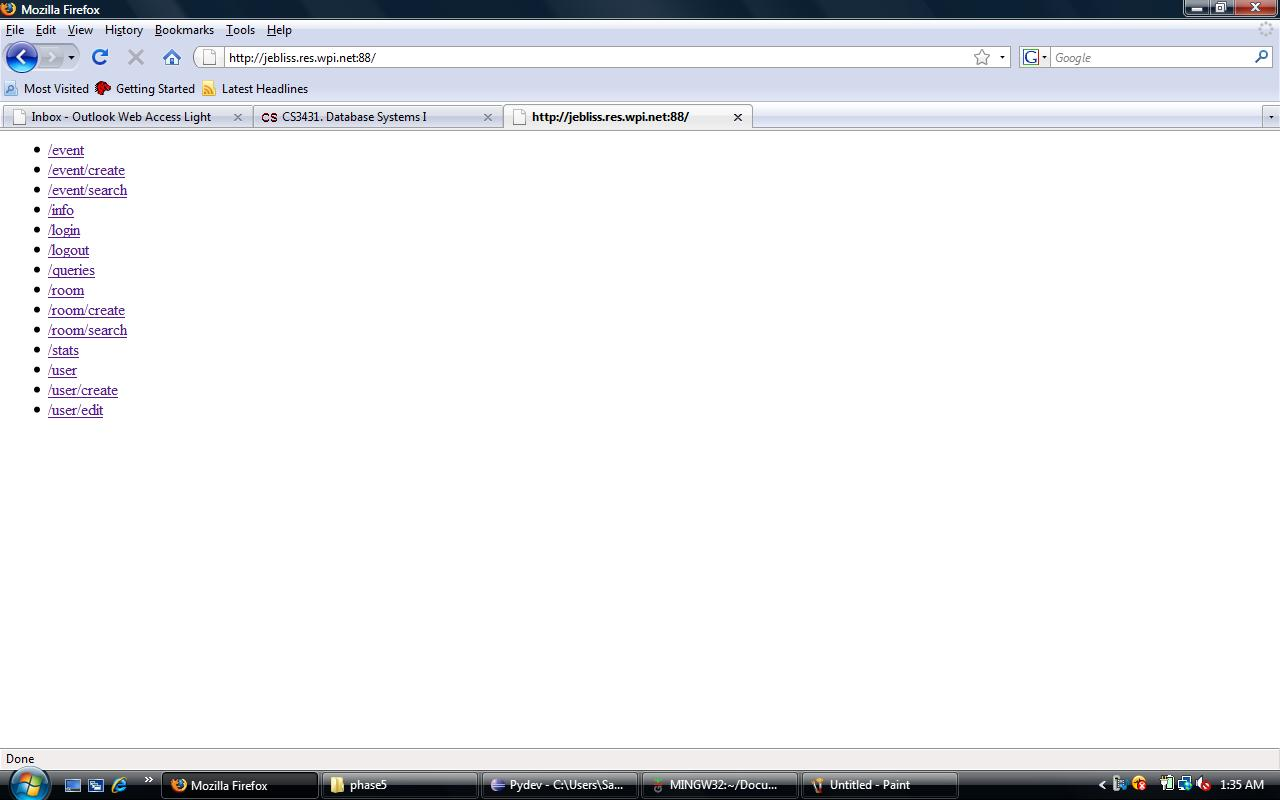
\includegraphics{\walkthrough\1.jpg}
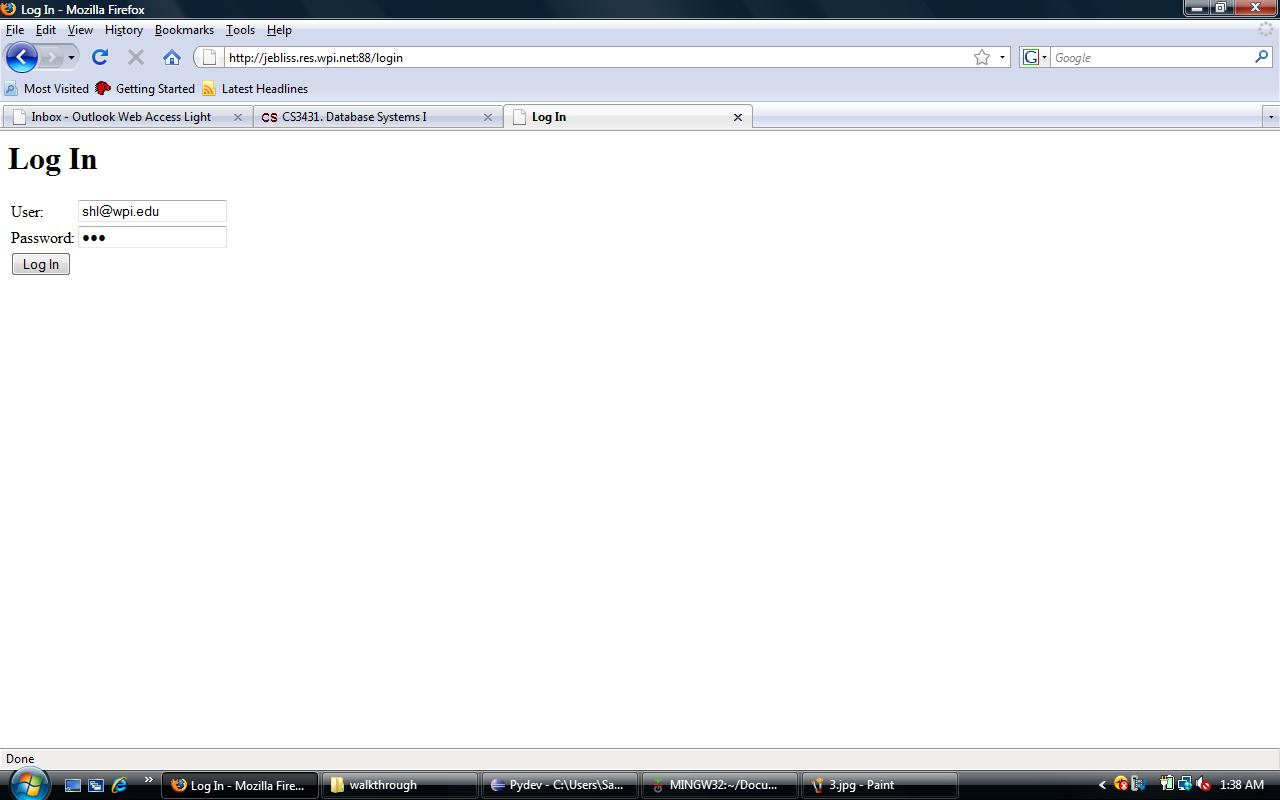
\includegraphics{\walkthrough\2.jpg}
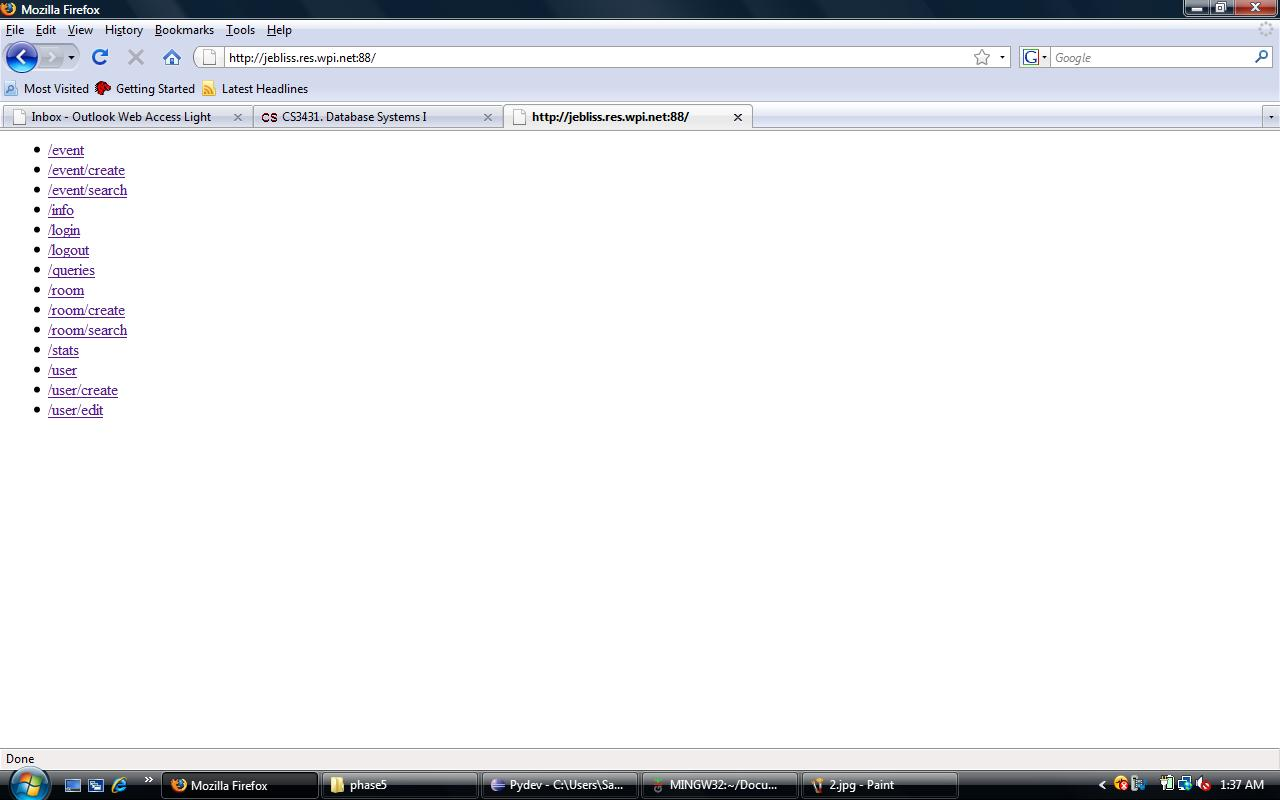
\includegraphics{\walkthrough\3.jpg}
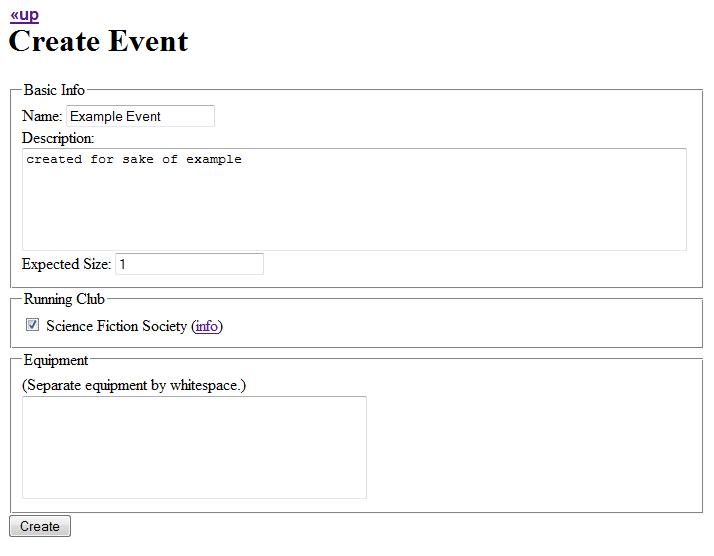
\includegraphics{\walkthrough\4.jpg}
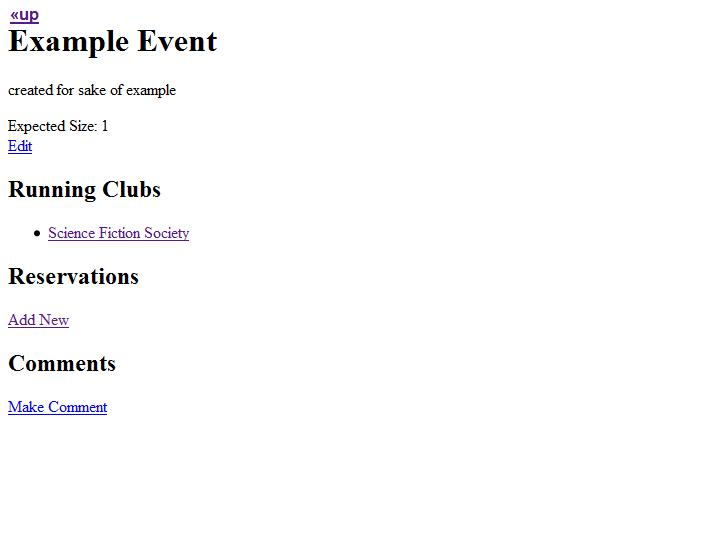
\includegraphics{\walkthrough\5.jpg}
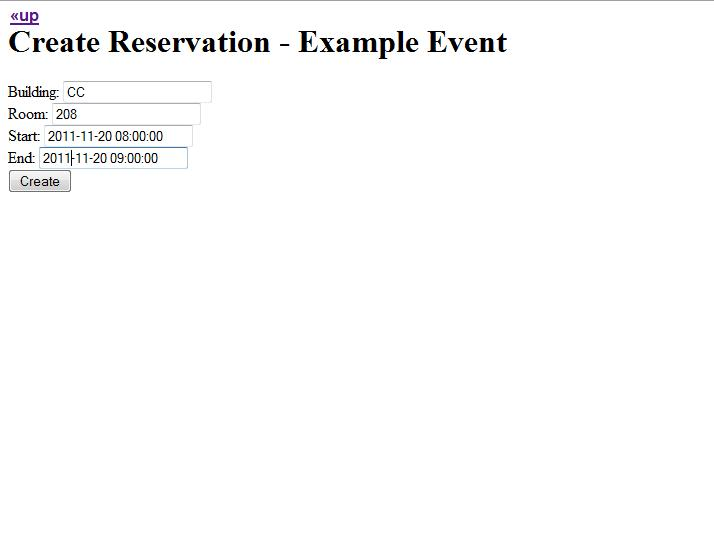
\includegraphics{\walkthrough\6.jpg}
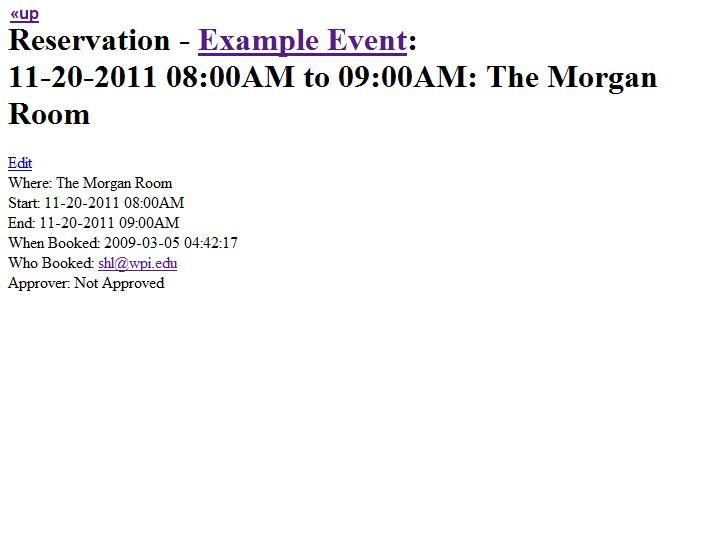
\includegraphics{\walkthrough\7.jpg}
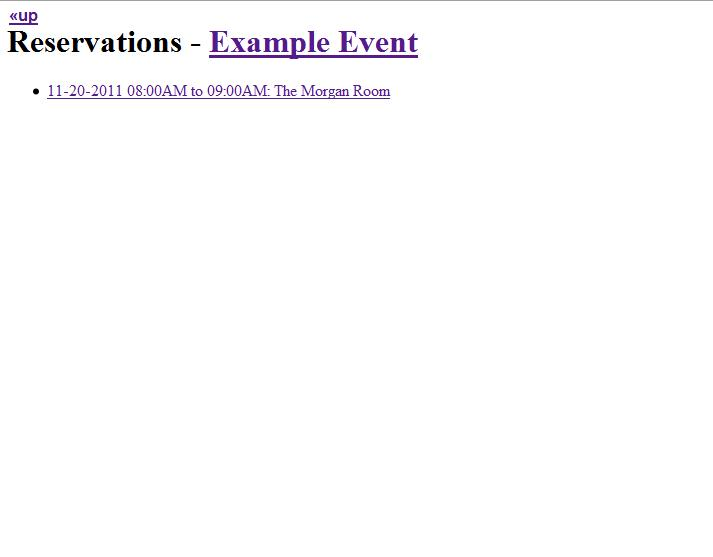
\includegraphics{\walkthrough\8.jpg}
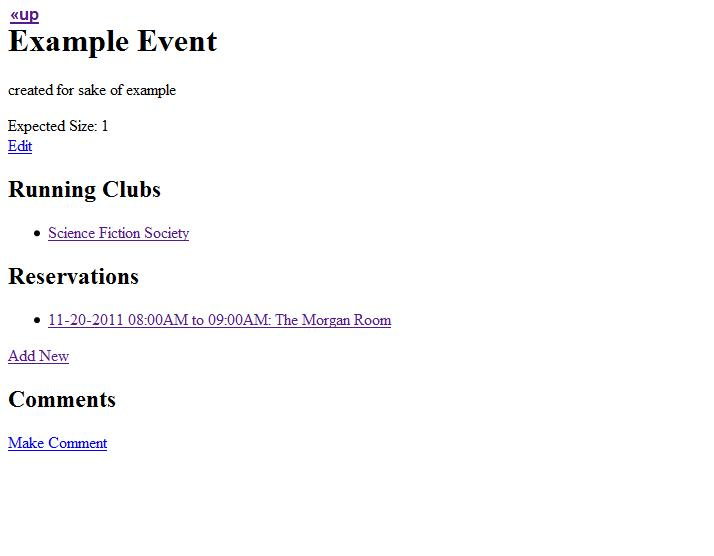
\includegraphics{\walkthrough\9.jpg}
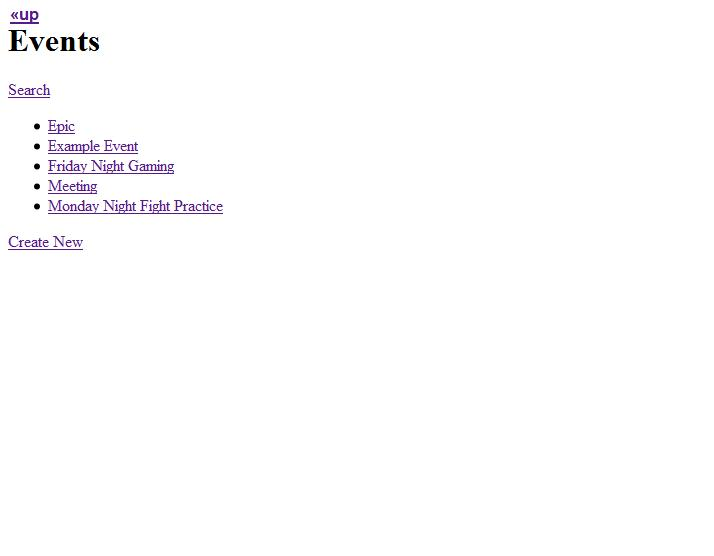
\includegraphics{\walkthrough\10.jpg}
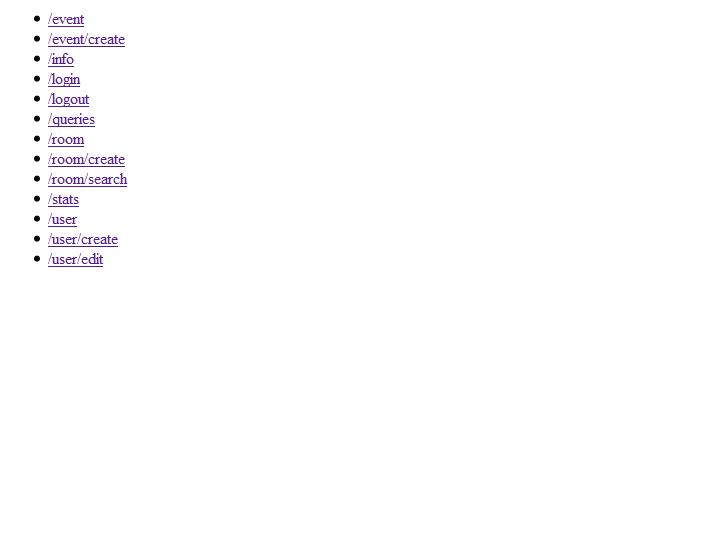
\includegraphics{\walkthrough\11.jpg}
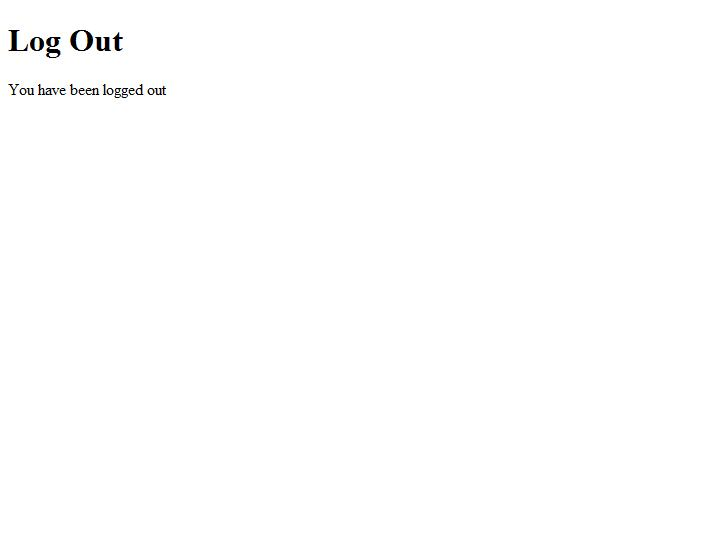
\includegraphics{\walkthrough\12.jpg}
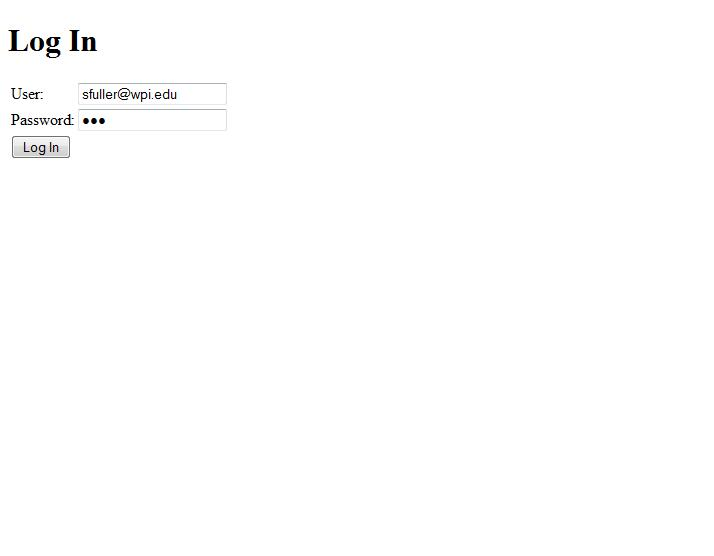
\includegraphics{\walkthrough\13.jpg}
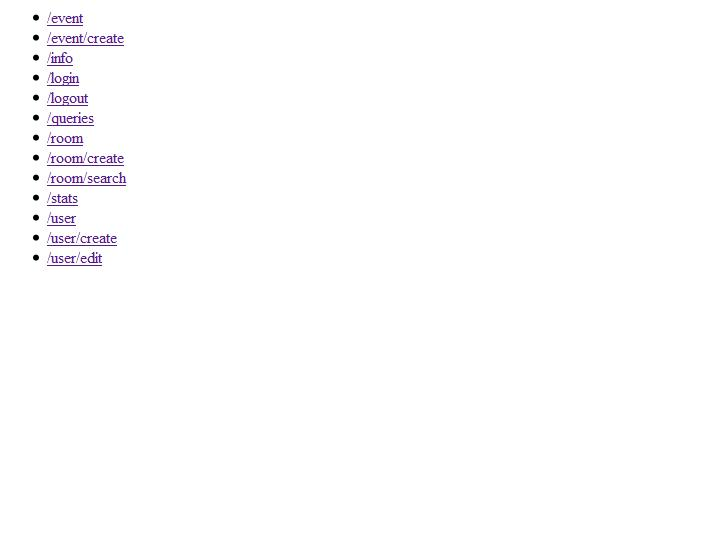
\includegraphics{\walkthrough\14.jpg}
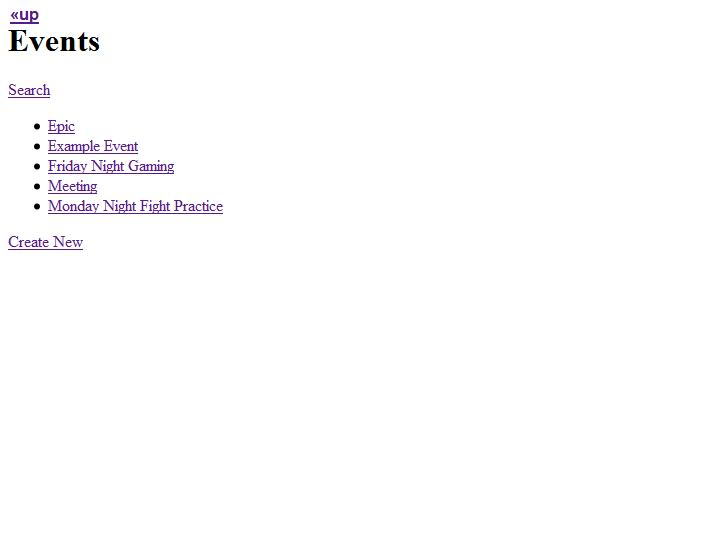
\includegraphics{\walkthrough\15.jpg}
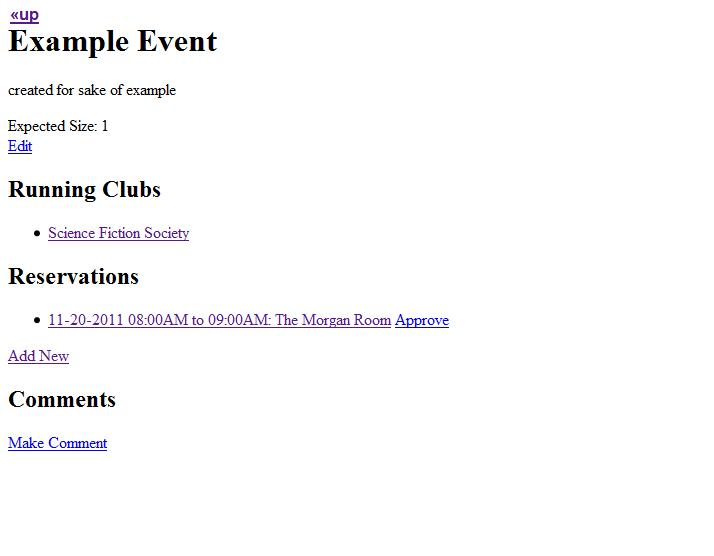
\includegraphics{\walkthrough\16.jpg}
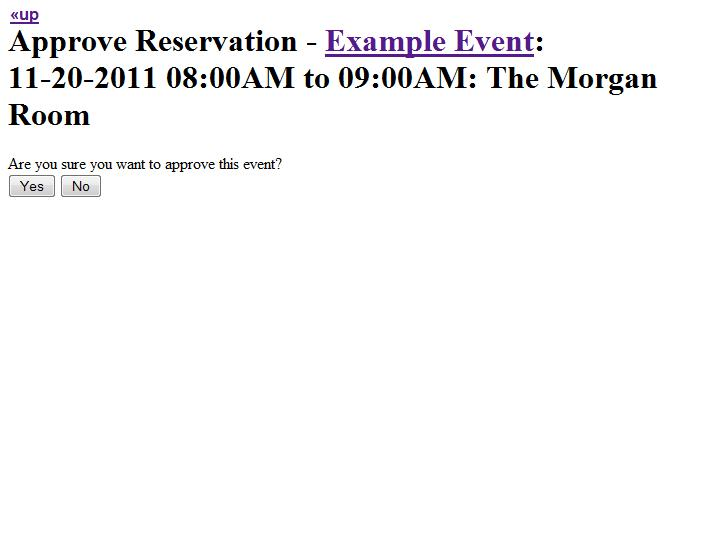
\includegraphics{\walkthrough\17.jpg}
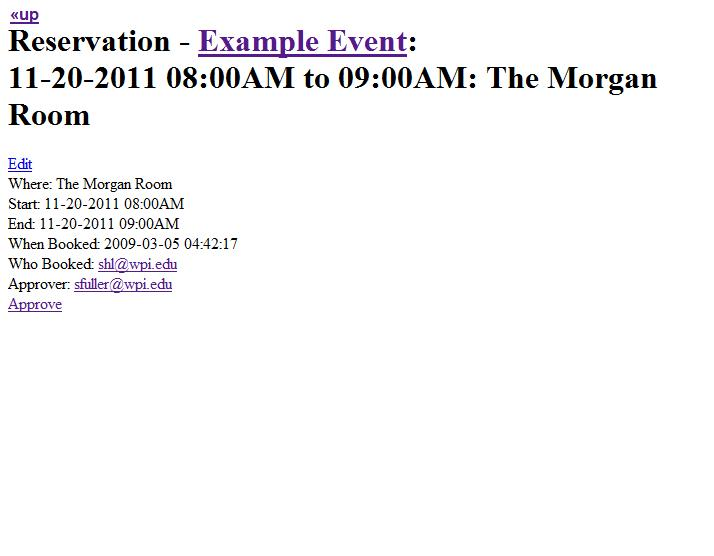
\includegraphics{\walkthrough\18.jpg}
% someone check this formating

\section{Division of Labor}
The project team met several times for this project phase. The devision of work on is as follows:

Sam:
Wrote the documentation.

Stephanie:
Wrote the system that deals with rooms.

Jamie:
Spearheaded system implementation. Has been working on it since phase 1.


\end{document}

